% !TEX root = ../main.tex

\chapter{Background}\label{ch:background}
Readers with a blockchain background may skip this chapter, as it covers foundational concepts that will be discussed in detail in the other chapters.

\section{Blockchain's Expanding Influence}
Blockchain is a distributed, untrusted network where participants (nodes) can freely connect or disconnect. Without the oversight of a central authority, all nodes collaborate to maintain data integrity through various consensus protocols (\eg Proof of Work (PoW), Proof of Stake (PoS), Proof of Burn (PoB), \etc). If one node encounters hardware or communication failures, other nodes seamlessly continue processing requests, as each maintains a full, synchronized copy of the data. Blockchain's significance extends beyond technical resilience. According to trusted advisories~\cite{Gartner, Reportlinker}, blockchain was expected to grow at an average rate of 51\% between 2016 and 2022, surpassing \$2 billion USD in revenue by 2022. With its expanding application scope and projected growth, blockchain is poised to become a foundational technology across multiple industries.

The global blockchain market was valued at \$3.0 billion in 2020 and is projected to reach \$39.7 billion by 2025, growing at a compound annual growth rate (CAGR) of 67.3\%~\cite{GrandViewResearch2020}. Financial services are leading the adoption, with banks expected to adopt blockchain solutions soon for payment and settlement systems. Moreover, decentralized finance (DeFi) has seen explosive growth, surpassing \$200 billion in total value locked (TVL) by 2021~\cite{MarketsandMarkets2020}, demonstrating the increasing usability of blockchain for applications such as lending, borrowing, and trading without intermediaries.

Furthermore, blockchain’s utility is expanding beyond finance. By 2025, it is estimated that 55\% of all healthcare applications will incorporate blockchain for securing patient records and enhancing data sharing~\cite{XcubeLabs2020}. Supply chain management is another domain rapidly integrating blockchain to ensure transparency and traceability. Major companies like Walmart and IBM have already adopted blockchain for tracking products from origin to retail~\cite{Sristy2021}.

\section{Ethereum's Smart Contract Ecosystem}
Out of 22 various implementations of the blockchain~\cite{builtin2024}, Ethereum~\cite{EIP150} is more widely accepted by the industry. It is a public blockchain proposed in 2013, deployed in 2015, and has the second largest market cap at the time of writing. It has a large development community which track enhancements and propose new ideas~\cite{CoinDesk20}. Ethereum enables decentralized applications to be deployed and executed on top of the blockchain. Smart contracts are essential component of the Ethereum and has been adopted widely by holding millions dollars worth of digital coins in form of ETH, ERC-20 tokens, Digital wallets and DeFi protocols.

Smart contracts are self-executing programs where the terms of the agreement are directly written into code. They automatically enforce and execute predefined rules and conditions without the need for intermediaries, ensuring transparency and reducing the risk of manipulation. In the Ethereum ecosystem, smart contracts are deployed on the blockchain, making them immutable and tamper-proof once published. Developers can use one of the high level programming languages in Ethereum (\eg Solidity, Vyper, \etc) to write smart contracts. These contracts can handle a wide range of transactions, from simple token transfers to complex decentralized applications (DApps). Their programmability allows developers to define various interactions, such as token exchanges, voting mechanisms, or multi-signature wallets, making them a cornerstone of Ethereum’s functionality.

Like other emerging technologies, security is an important aspect of smart contracts. Previous research discovered that at about 45\% of existing smart contracts on the Ethereum are vulnerable~\cite{SmartContractSecurity}. The development of smart contracts has been proven to be error-prone, and as a result, smart contracts are often riddled with security vulnerabilities. One of the major smart contract hacks was due to TheDAO bug, which caused a loss of 60 million US dollars in June 2016~\cite{TheDAOCoinDesk}. Similar to other programming languages, smart contracts' codes can be exploited by an adversary (\ie Miner, external users and other contracts) to manipulate executions and gain profit. Some smart contracts have kept millions of dollars, which could be enough to incentivize adversaries to exploit vulnerabilities.

\begin{example}
	Aave is a decentralized lending protocol, with a total value locked (TVL) consistently exceeding \$6 billion. Users can earn interest by supplying assets or take out loans by borrowing crypto with their deposits as collateral. As another example, Uniswap, one of the largest decentralized exchanges (DEX), has a TVL of approximately \$3.7 billion and allows users to trade directly from their wallets~\cite{theblock2024}.
\end{example}

\section{Decentralized Apps and ERC-20 Tokens}
Migrating applications from centralized to decentralized architecture can solve many issues such as single point of failure, hardware and maintenance costs, and data security. This type of application is distributed over an untrusted network and leverage smart contracts to run codes on the blockchain. Tokens are subset of smart contracts and security is particularly important given that many tokens have considerable market capitalization. As tokens can be held by commercial firms, in addition to individuals, and firms need audited financial statements in certain circumstances, the correctness of the smart contract issuing the tokens is now in the purview of professional auditors.

Ethereum allows DApps to accept and use ETH as its protocol-level cryptocurrency or issue their own custom tokens with a variety of intents (\eg In-app purchase, Interoperability with other dApps, Representing digital assets, \etc). Tokens might be currencies with different properties than ETH, they may be required for access to a dApp's functionality or they might represent ownership of some off-blockchain asset. It is beneficial to have interoperable tokens with other dApps and off-blockchain webapps, such as exchange services that allow tokens to be traded. In this regard, the Ethereum community accepted a popular token standard called ERC-20~\cite{Interface}. As shown in Figure \ref{fig:interface}, ERC-20 is an interface that defines abstract methods (name, parameters, return types) and provides guidelines on how the methods should be implemented, however it does not provide an actual concrete implementation. Developers have the flexibility of implementing ERC-20 methods according to the needs of their dApps, or even expand it to offer new functionalities.

\begin{figure}[t]
	\centering
	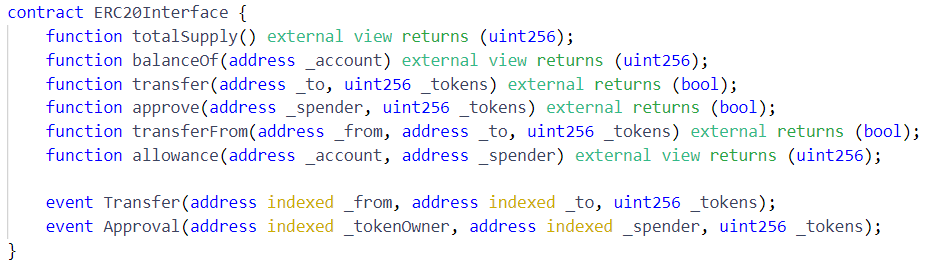
\includegraphics[width=\textwidth,keepaspectratio]{interface.png}
	\caption{The ERC-20 interface in Solidity defines a set of functions that any contract implementing the ERC-20 standard must include. These functions ensure interoperability and compatibility with other ERC-20 compliant contracts, wallets, exchanges, and decentralized applications.}
	\label{fig:interface}
\end{figure}

While numerous ERC-20 extensions or replacements have been proposed (\eg ERC-721, ERC-777, ERC-1155, \etc), ERC-20 remains prominent. Of the 2.5M smart contracts on the Ethereum network, 260K are tokens~\cite{TokenTracker}. 98\% of these tokens are ERC-20 tokens, demonstrating their widespread acceptance by the industry, smart contract developers and the Ethereum community. As shown in Figure \ref{fig:layers}, among the layers of the Ethereum blockchain, ERC-20 tokens fall under the \textit{Contract layer} in which back-end of DApps are executed.

\begin{figure}[t]
	\centering
	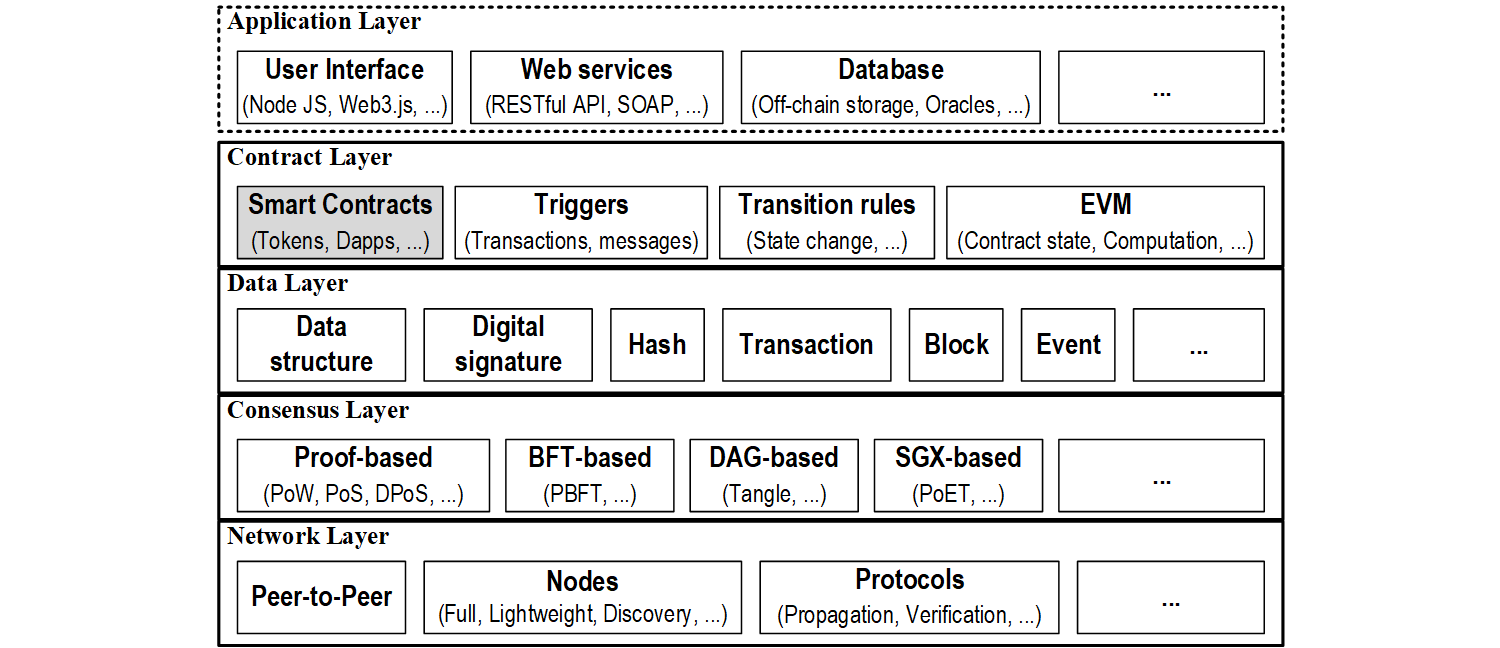
\includegraphics[width=\textwidth,keepaspectratio]{blockchain.png}
	\caption{Smart contracts generally exist at the contract layer, leveraging the underlying consensus mechanisms for secure execution and state changes. The \textit{Contract Layer} can be considered a sublayer of the \textit{Application Layer}, focusing on how smart contracts execute and interact with blockchain transactions.}
	\label{fig:layers}
\end{figure}

\section{Complexity of Leveraged Tokens}
\subsection{Models and Dynamic}
A typical Exchange-Traded Fund (ETF) is a weighted basket of stocks from firms with a common characteristic (e.g., they all operate in a specific sector or have a high market capitalization). The issuer splits the basket into shares, which are bought and sold on exchanges just like individual stocks~\cite{liebi2020effect}.
\begin{example}
	One of the most widely traded ETFs is the \textsl{SPDR S\&P500 ETF}, with the ticker symbol \textsl{SPY}. It is issued by SSGA\anote{ssga} and holds a basket of stocks from nearly 500 publicly traded companies that are included in the S\&P500\anote{SP500} index. The S\&P500 index has globally served as a gauge for the performance of the U.S. stock market as a whole, due to its depth and diversity. Since SPY tracks the S\&P500 index, investors can gain broad exposure and diversify their investment risk across the stock performance of 500 companies in 11 sectors without the logistics or starting capital required to buy shares in all these companies.
\end{example}

Leveraged ETFs (LETFs) were introduced in 2006 and are ETFs designed to amplify the daily performance of the underlying basket (more on leverage in Section \ref{subsec:leveragedproduct}).\anote{underlying} Inverse LETFs aim to achieve a return that is a multiple of the inverse of the underlying asset’s daily performance~\cite{hill2009understanding,cheng2009dynamics,SEC}. Many investors alternatively refer to LETFs and inverse LETFs as ``Bullish'' and ``Bearish'' LETFs, respectively, reflecting their short-term sentiment on future price movements.
\begin{example}
	\textsl{Direxion Daily S\&P500 Bull 3x ETF (SPXL)} is a 3x (three times) LETF that seeks to deliver triple the daily performance of the S\&P500. It magnifies each 1\% gain in the S\&P500 index into a 3\% gain and loses 3\% for every 1\% drop in the index. \textsl{Direxion Daily S\&P500 Bear 3x ETF (SPXS)} delivers triple the opposite daily performance of the S\&P500 index. If the S\&P500 index depreciates by 1\%, SPXS gains 3\%, and vice versa~\cite{wided2019properties,lettau2018exchange}.
\end{example}

A Leveraged Token (LVT) in the cryptocurrency and crypto-asset (``crypto'') market can be compared to a Leveraged ETF (LETF) in the traditional financial market. Similar to LETFs, LVTs use leveraged products available in the crypto market to outperform the underlying asset’s return on a daily basis. While the majority of LETFs are actively managed funds\anote{active}, LVTs employ one of three management models: (i) centralized, (ii) decentralized, and (iii) hybrid. 

Centralized LVTs are primarily managed by crypto exchanges and can be purchased on the spot market or directly from the issuer. Decentralized LVTs operate on-chain and can be traded by interacting directly with the smart contract. Hybrid LVTs are essentially decentralized LVTs that are traded on centralized crypto exchanges. Users prefer centralized exchanges for their user-friendly interfaces, continuous-time order books (rather than automated market makers, which are the only trading mechanism efficient enough to run on-chain), and increased liquidity due to aggregated buy and sell orders.\anote{liquidity} However, this model introduces certain disadvantages resulting from the combination of centralized and decentralized systems (\eg functional complexities, security concerns, custodial risks, \etc.).

\begin{example}
	An issuer may offer BTC3L/BTC3S as a pair of LVTs tracking Bitcoin (BTC) as the underlying asset. A Bitcoin futures contract (BTC-Perp\anote{btc-perp}) can be used as the leveraged product to outperform Bitcoin in the short term. The number three in the LVT name represents the multiplier (triple-leveraged), while L/S stands for going long/short on the market.\anote{long-short} BTC3L gains 3\% when the price of Bitcoin rises by 1\%, and loses 3\% for every 1\% price drop. Conversely, when Bitcoin drops by 1\%, BTC3S gains 3\%, and loses 3\% for every 1\% price rise.
\end{example}

\subsection{Volatility drag}\label{appx:voldrag}
Volatility measures the rate of change in the value of an asset. The value of a highly volatile asset can potentially spread out over a larger range of values and change dramatically over a short period of time in either direction. Conversely, the value of a low-volatility asset does not fluctuate significantly and tends to be more stable. In the equity market, for instance, when the price of a specific stock rises or falls by more than 1\% over a sustained period of time, it is considered a volatile stock, especially when compared to historical price movements~\cite{Investo_Volatility}.

\textsl{Volatility drag} represents the rate at which the value of investments dissipates\anote{vol-drag}. As volatility increases and positions are held open for a longer period, the drag imposed by volatility accelerates, making it more destructive to the overall value of the investment~\cite{tsalikis2019can, SeekingAlpha_Volatility}. A similar effect occurs in LVTs, which impacts return on investment.

\ExecuteMetaData[sections/tables]{tab-voldrag}

\begin{example}
	The performance of 3x and 5x Long/Short BTC tokens with a \$200 initial investment is compared in a volatile market. The assumption in Table \ref{tab:voldrag} is a 5\% BTC price increase on day 1, followed by another 5\% increase on day 2, and then a 10\% drop on day 3, continuing in this pattern. Mathematically, two 5\% increases on days 1 and 2 should be offset by a 10\% drop on day 3. However, the math does not align as expected due to accumulated profit or loss. The price of a non-leveraged BTC position increases by 5\% from \$200 to \$210 on day 1 and by another 5\% from \$210 to \$220.5 on day 2 (a 10.25\% gain after 2 days). A 10\% drop on day 3 from \$220.5 to \$198.45 results in a position that is -0.78\% lower than the initial investment, making the overall return negative. 
	
	This loss is -7.43\% and -21.88\% of the initial investment for BTC3L and BTC5L, respectively. Investors would expect better performance from BTC3S and BTC5S on the short side. However, due to accumulated losses in the first two days, they close at -6.08\% and -15.63\% lower than the starting value. Even after a week, when the initial investment has nearly reached the break-even point, all LVTs remain negative regardless of their leverage and direction (See Figure \ref{fig:voldrag}).
	
	\begin{figure}[t]
		\centering
		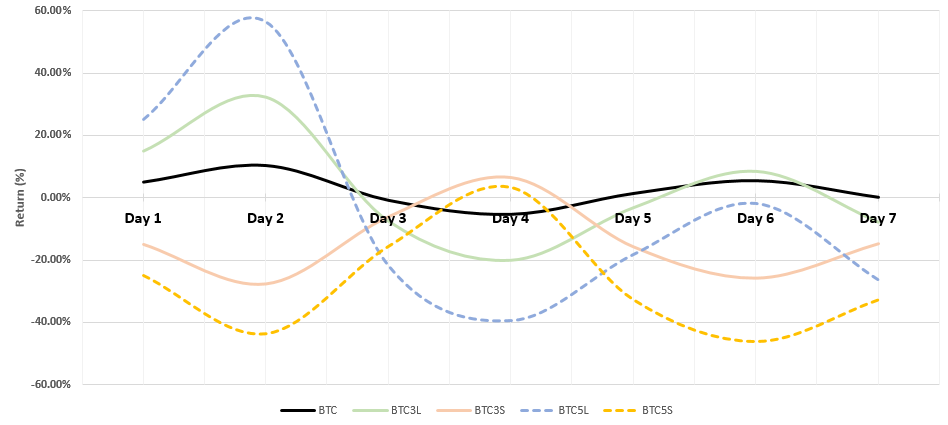
\includegraphics[width=0.9\textwidth,keepaspectratio]{voldrag.png}
		\caption{LVT returns during a volatile week: the value of the initial investment (BTC in black) reached the breakeven point on day 7, but the returns of all LVTs remained negative due to the impact of volatility drag.}
		\label{fig:voldrag}
	\end{figure}
\end{example}

As the above example suggests, volatility negatively impacts the performance of LVT investments over time, as previously discussed in the case of LETFs~\cite{giese2010performance, trainor2011daily}. While volatility can be beneficial in the short term, compounded daily returns produce unexpected mathematical outcomes. Investors would have made some profits if they had closed their positions on the first or second day, but holding the position through the third day would have resulted in a loss. To minimize the impact of volatility drag on LVTs, it is better to use them as short-term investments in markets with strong trends and momentum.


\subsection{Leverage Products}
LVTs derive their value from a leveraged fund, which in turn is based on a leveraged product. This leveraged product typically originates from either the \textit{Crypto derivatives market} or the \textit{DeFi lending market} (see Figure \ref{fig:markets} for possible options in each market). In the \textit{derivatives market}, Perpetual futures (Perps)\anote{perps} are particularly popular due to their flexible nature. Since Perps have no expiration date, they can be held indefinitely, with the added benefit of allowing LVTs to take leveraged positions without concerns about contract expiration or rollover. This is especially appealing for users seeking higher returns, though the inherent risk of leverage can amplify losses as well. 

Conversely, the \textit{DeFi lending market} offers a more conservative approach, allowing LVTs to borrow assets through decentralized platforms such as Aave and Compound.\anote{lending} While perpetual futures offer higher leverage and come with greater risk, lending protocols provide lower leverage with reduced risk. The choice between using perpetual futures or lending protocols for LVTs is largely determined by the specific design and intended purpose of the token, as well as the user’s risk tolerance.

\begin{figure}[t]
	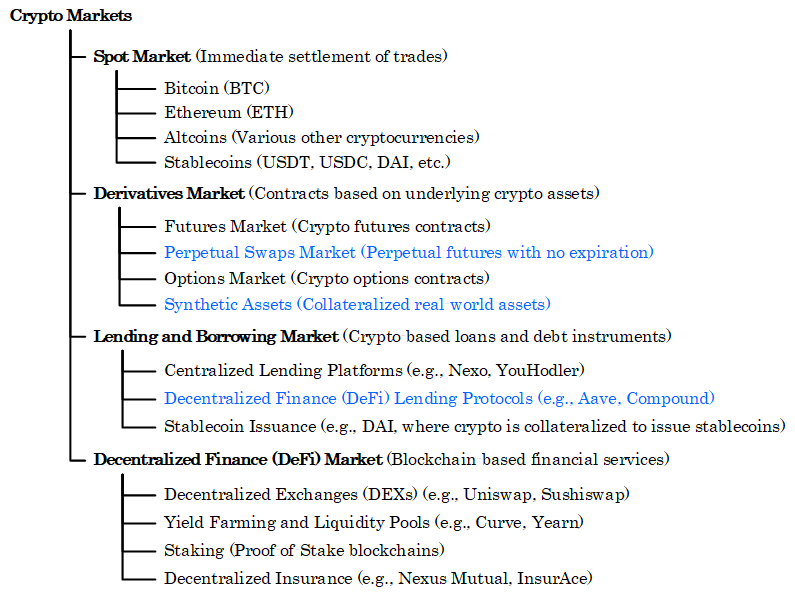
\includegraphics[width=\textwidth,keepaspectratio]{markets.png}
	\caption{A hierarchy of various types of crypto markets and instruments, delineates the positions of the Futures and Lending markets (in blue).}
	\label{fig:markets}
\end{figure}

LVTs simplify the complexities of maintaining a leveraged position for users, such as constant monitoring, manual position adjustments, and margin management. But how do LVTs generate leverage on behalf of users? Both the crypto derivatives and DeFi lending markets offer effective ways to achieve desired leverage factors for LVTs. With relatively modest leverage limits in LVTs (typically up to 5x), obtaining leverage is feasible in either market. In derivatives markets, leverage can be generated using dated futures, perpetual contracts, or synthetic assets. In DeFi lending market, leverage can be achieved by borrowing funds against collateral and reinvesting them to increase exposure (see the highlighted options in Figure \ref{fig:markets}.). 

When choosing between these leveraged products, key factors include risk tolerance, investment time horizon (short-term or long-term), and the depth of liquidity provided by the underlying platform.

\subsubsection{Dated Futures}
They can be used in LVTs to provide leverage till specific expiration date.\anote{dated} Unlike perpetual futures, which have no expiration date, dated futures contracts require the position to be settled or rolled over by the expiration date. LVTs using dated futures must roll over contracts before their expiration date to maintain the leveraged exposure. The smart contract managing the LVT sells the expiring contracts and simultaneously buys new contracts with a later expiration date. This process ensures that the fund continues to maintain its leveraged exposure to the underlying asset without interruption. 

The rollover process can sometimes result in minor costs or changes in the leverage ratio due to differences in prices between the expiring and new contracts (known as "roll yield"). If the futures market is in Contango\anote{contango}, the roll yield is negative, and the LVT effectively pays a premium to maintain its leveraged positions. In Backwardation\anote{backwardation}, the roll yield is positive, and the LVT benefits from the lower price of the new contract. There is also a risk of the smart contract failing to renew or roll over the expired futures. This may lead to several potential consequences, such as loss of leverage exposure, token devaluation, and potential liquidation in DEXs if holders rush to sell off the under-collateralized tokens.

\subsubsection{Perpetual Futures}
They can be used as leveraged products in LVTs without the need to settle or roll over at a specific future date, which reduces slippage and costs associated with dated futures. Additionally, they differ from dated futures in terms of funding fees (see section \ref{appx:funding} for more details). However, a drawback of perpetual futures is their sensitivity to market volatility, which can lead to rapid changes in maintenance margin and increase the likelihood of forced liquidation. This makes them more suitable for short-term investments rather than for buy-and-hold use cases.

\subsubsection{Automated Stacking}\label{appx:looping}
Looped positions (\ie borrowing, re-depositing, and borrowing again) on fixed-rate\anote{fixed} lending markets can be seen as somewhat analogous to dated futures contracts. Comparatively, variable-rate\anote{dynamic} positions on lending markets can be interpreted as the funding rate of the position, which in turn can be seen as a perpetual futures.

\subsubsection{Synthetic Assets}
These assets allow users to gain exposure to the price movement of various assets without directly owning them. Synthetic assets can track the value of fiat currencies, stocks, commodities, cryptocurrencies, or other financial derivatives. Synthetic assets are usually backed by collateral (often in crypto) to ensure they maintain their value. For example, Synthetix protocol use collateralized debt to mint synthetic assets. They enable users to create tokens that track the value of real-world assets.

\subsubsection{Summary of Key Differences}\label{appx:summary}
An LVT is primarily utilized by investors seeking a tokenized fund that simplifies the management of leveraged positions while providing liquidation protection. Identifying the target user is essential when choosing the appropriate leveraged product before issuing LVTs. For long-term investors, the debt market is generally more cost-effective due to reduced daily token depreciation. In contrast, futures are better suited for short-term investors, as outlined below.
\begin{itemize}
	\item \textit{Perpetual futures:} Best for short-term leveraged tokens that require frequent rebalancing. Their advantage lies in their flexibility and potential for high leverage in both short and long directions.
	
	\item \textit{Debt-based leveraged positions:} This method is better suited for stable or moderate leverage but carries risks of liquidation and fluctuating interest rates. Additionally, the maximum leverage is limited by the lender's LTV ratio, which varies across blockchains. Moreover, creating short LVTs is more challenging than long positions due to the requirement for overcollateralization (see the short token process in Figure \ref{fig:looping}).
	
	\item \textit{Synthetic assets:} While synthetic assets provide leveraged exposure in a fully decentralized manner, they come with potential drawbacks, such as overcollateralization and concerns over oracle accuracy.
\end{itemize}
The advantages and disadvantages of each leveraged product across key factors depend on the investment horizon and issuer preferences. Since LVTs are primarily used by short-term traders aiming to realize profits within the same trading day, perpetual futures are the most suitable option for inclusion in LVTs. However, issuers with a long-term investment horizon may opt for debt-based LVTs, which have distinct characteristics discussed in the upcoming chapters.

\subsection{Key Factors in Crypto Futures Market}\label{appx:futures}
As mentioned, futures contracts are commitments to buy or sell a specific cryptocurrency at a predetermined price on a future date. The Crypto Futures Market is a marketplace where these contracts are bought and sold, facilitating speculation on crypto price movements. Futures often involves the use of leverage, which allows traders to increase their exposure with less initial capital. Additionally, it enables hedging and speculation on future price movements. Perpetual Futures contracts (Perps) are a dominant type of contract in this market, allowing users to maintain a leveraged position indefinitely without an expiration date. The risks associated with Perps are largely tied to the \textsl{Funding Rate} and the possibility of \textsl{Liquidation}.

\subsubsection{Funding Fee}\label{appx:funding}
Traditional futures contracts have an expiration date known as the delivery date. Futures prices converge with the spot price on this date. Before that, the market can be in one of two conditions: Contango or Backwardation~\cite{cme2020contango}. Contango and Backwardation describe the price relationship between the spot and futures contracts. When the market is in Contango, futures are traded at a premium to the spot price (\ie they are more expensive). When the market is in Backwardation, futures are traded at a discount to the spot price (\ie they are cheaper than the spot price)~\cite{abd2019contango}. Contango or Backwardation may occur due to shocks in supply or demand, carrying costs, geopolitical situations, pandemics, etc. Ultimately, traditional futures prices converge with the spot price by the delivery date (see Figure \ref{fig:fundingfee}).

\begin{figure}[t]
	\centering
	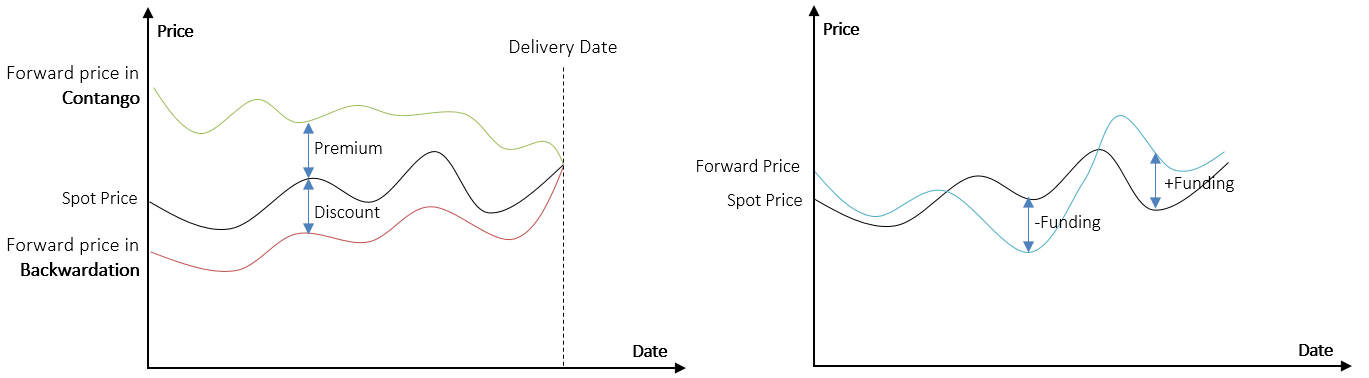
\includegraphics[width=\textwidth,keepaspectratio]{fundingfee.png}
	\caption{Contango or Backwardation conditions in the traditional futures market with a specific delivery date (left image). Price convergence over time in perpetual futures contracts, influenced by the funding rate (right image).}
	\label{fig:fundingfee}
\end{figure}

In crypto perpetual contracts, there is no delivery date, but the futures price still needs to settle against the spot price. At times, one side of the market becomes more aggressive, causing a disparity between spot and futures prices. To keep these prices aligned, a funding rate component is added to crypto futures. Only open positions are subject to funding payments or receipts at specific times (usually every 8 hours). If a position is closed before the funding exchange, traders do not pay or receive the funding fee. The funding fee can significantly impact high-leverage positions, potentially even leading to liquidation when paying for funding~\cite{Poloniex_FundingFee}.

Funding fee represents a periodic payment exchanged between traders holding long and short positions, intended to keep the contract's price (\(P_t\)) aligned with the underlying asset's spot price (\(S_t\)). When \(P_t > S_t\), the perpetual contract is trading at a premium, typically indicating higher demand for long positions. Conversely, when \(P_t < S_t\), the contract is trading at a discount, suggesting higher demand for short positions. The funding fee is a mechanism designed to encourage traders to take the opposite position and correct the imbalance. Let \(F_t\) represent the funding rate at time \(t\) expressed by:
\begin{equation}\label{eq:funding1}
	F_t = \alpha \left( \frac{P_t - S_t}{S_t} \right) + \beta \left( r_f - r_c \right)
\end{equation}
where \( r_f \) denotes the interest rate of the fiat currency and \( r_c \) denotes the interest rate of the cryptocurrency. Subsequently, \((\frac{P_t - S_t}{S_t})\) and \((r_f - r_c)\) are the "premium or discount" and "interest rate" components, with weighted coefficients \( \alpha \) and \( \beta \), respectively. Both \( \alpha \) and \( \beta \) are adjustable parameters that exchanges or DeFi platforms might calibrate based on market conditions, volatility, and the desired level of price convergence between the perpetual contract and the spot market. For instance, a high \( \alpha \) might be used in a highly volatile market to quickly correct large premiums or discounts, while a high \( \beta \) might be more relevant in a market where the cost of capital (borrowing rates, staking yields, etc.) is highly volatile~\cite{Binance_Funding,BitMEX_Funding}.

\subsubsection{Liquidation}\label{subsec:liquidation}
It occurs when futures positions are automatically closed due to insufficient maintenance margin. Liquidation is primarily driven by:
\begin{itemize}
	\item \textsl{Adverse price movements:} When the market price moves against the position, it leads to a decline in notional value and a reduction in account equity.

	\item \textsl{Unfavorable funding rates:} When the funding rate is negative for the position, resulting in a continuous deduction from the margin balance. Over time, if the funding rate expenses erode the margin to the point where it falls below the maintenance margin threshold (usually 5-10\% of the initial margin), liquidation occurs by the exchange without user consent.
\end{itemize}
The liquidation process is triggered when the price of the underlying asset falls below the \textit{liquidation price}, at which the value of the initial margin is no longer adequate. The liquidation price ($P_{Liq}$) can be calculated as \(P_{Liq} = P_{Ent} \times \left( 1 - \frac{1 - \mu}{\lambda} \right)\), where \(\lambda\) represents the leverage of the position (negative for shorts), \(P_{Ent}\) is the entry price and \(\mu\) is maintenance margin in percentage.

\begin{example}\label{ex:funding2}
	Bob opens a 10x long BTC/USDT Perps at \(P_{Ent} = \$30K\) with an initial margin of \$3K and a maintenance margin of \(\mu = 5\%\). Since this is a 10x position (\(\lambda = 10\)), it requires 10 times less capital than the full position value. The liquidation price is calculated as \(P_{Liq} = \$30K \times ( 1 - \frac{1 - 5\%}{10} ) = \$30K \times 0.905 = \$27,150\), at which point Bob’s position would automatically be closed by the exchange, and his initial margin of \$3K would be used to cover the losses. In other words, Bob loses his entire initial investment as a result of liquidation.
\end{example}